\chapter{Teoretické východiská}

Táto kapitola zavádza pojmy, ktoré budú použité v ďalších častiach práce. Cieľom ešte nie je opisovať konkrétnu implementáciu agenta ani výsledky experimentov. Najprv potrebujeme spoločný slovník: čo je agent, prostredie, pozorovanie, akcia, politika správania sa agenta, odmena, neurónová sieť a optimalizačný algoritmus. Až potom má zmysel ukázať, ako sa tieto pojmy spájajú v konkrétnom riešení autonómneho vodiča.

Teoretická časť je preto písaná od všeobecného k špecifickejšiemu. Najprv sa pozrieme na umelú inteligenciu ako na problém rozhodovania v prostredí. Následne zavedieme formálny model agenta a jeho politiky správania sa. Na tento základ potom nadviaže hodnotenie správania, neurónové siete a metódy učenia, ktoré hľadajú vhodné parametre rozhodovacej funkcie.

\section{Umelá inteligencia a autonómne rozhodovanie}

Umelá inteligencia je široký pojem a v rôznych obdobiach sa na ňu kládol iný dôraz. Historicky sa často spájala s otázkou, či stroj dokáže prejavovať správanie, ktoré by sme u človeka označili za inteligentné \cite{turing1950computing}. Pre potreby tejto práce je však užitočnejší praktickejší pohľad: inteligentný systém budeme chápať ako systém, ktorý vníma svoje prostredie a volí akcie tak, aby dosahoval zadaný cieľ. Podobne definujú inteligentného agenta aj Russell a Norvig, ktorí zdôrazňujú dvojicu vnímanie prostredia a konanie v prostredí \cite{russell_norvig_aima2021}.

\paragraph{Riadenie ako sekvenčné rozhodovanie.}
Tento pohľad je vhodný najmä pri autonómnom riadení. Agent nemusí mať vedomie ani rozumieť svetu tak ako človek. Stačí, aby mal informácie o aktuálnej situácii, vedel zvoliť akciu a jeho správanie bolo možné hodnotiť podľa toho, či sa približuje k cieľu. Pri riadení vozidla môže byť cieľom napríklad bezpečne pokračovať po ceste, dostať sa do cieľa alebo prejsť trať za čo najkratší čas. Dôležité je, že agent nerieši jeden izolovaný výpočet. Rozhoduje sa postupne a každá jeho akcia ovplyvní situáciu, v ktorej sa bude rozhodovať neskôr.

\paragraph{Pravidlový systém a učiaci sa systém.}
Z tohto dôvodu je vhodné odlíšiť pravidlový systém od systému, ktorý sa učí. Pravidlový systém má správanie ručne opísané vopred. Autor systému doň zapíše podmienky a reakcie, napríklad čo má agent urobiť, ak sa pred ním nachádza prekážka. Takýto prístup môže byť čitateľný a dobre kontrolovateľný, ale pri zložitejšom prostredí môže byť krehký. Systém učený zo skúsenosti má namiesto pevne napísaných pravidiel parametre, ktoré sa menia podľa dát alebo podľa hodnotenia správania. Výhodou je, že takéto správanie nemusí byť celé ručne navrhnuté. Nevýhodou je, že potrebujeme vhodný spôsob učenia a vhodné hodnotenie, inak sa systém môže naučiť niečo iné, než sme zamýšľali.

Autonómne rozhodovanie je preto prirodzene sekvenčný problém. Agent v čase pozoruje prostredie, zvolí akciu, prostredie sa zmení a proces pokračuje. Rovnaká akcia nemusí mať vždy rovnaký význam, pretože závisí od stavu, v ktorom bola vykonaná. V riadiacich úlohách je táto vlastnosť obzvlášť výrazná. Jemná korekcia smeru môže byť pri nízkej rýchlosti bezpečná, ale pri vysokej rýchlosti môže zásadne zmeniť budúcu trajektóriu. Už na tejto úrovni teda vzniká hlavná otázka práce: ako nájsť rozhodovaciu funkciu, ktorá v každom kroku z dostupných informácií vyberie vhodnú akciu.

\section{Agent, prostredie a politika správania sa agenta}

Základný model sekvenčného rozhodovania pozostáva z agenta a prostredia. Prostredie označuje časť sveta, v ktorej sa agent nachádza a ktorú môže svojimi akciami ovplyvňovať. Agent je systém, ktorý z prostredia získava informácie a na ich základe volí akcie. Tento opis je zámerne všeobecný. Agentom môže byť robot, program ovládajúci postavu v hre, model obchodujúci na trhu alebo vodič vo virtuálnom pretekárskom prostredí.

\paragraph{Stav, pozorovanie a akcia.}
V diskrétnom čase môžeme interakciu zapísať nasledovne. V kroku $t$ sa prostredie nachádza v stave
\[
    s_t \in \mathcal{S},
\]
kde $\mathcal{S}$ je množina všetkých možných stavov. Agent nemusí mať prístup k celému skutočnému stavu. Často dostáva iba pozorovanie
\[
    o_t \in \mathcal{O},
\]
kde $\mathcal{O}$ je množina pozorovaní. Na základe tohto pozorovania zvolí akciu
\[
    a_t \in \mathcal{A},
\]
kde $\mathcal{A}$ je množina akcií, ktoré môže agent vykonať. Prostredie potom prejde do nového stavu. V stochastickom prípade tento prechod opisujeme pravdepodobnosťou
\[
    s_{t+1} \sim P(\cdot \mid s_t, a_t),
\]
teda nový stav sa vyberá podľa prechodového rozdelenia podmieneného aktuálnym stavom a akciou. V deterministickom prípade môžeme prechod zapísať jednoduchšie ako
\[
    s_{t+1} = f(s_t, a_t).
\]
Rovnakú myšlienku môžeme čítať aj ako prechod zo stavu $s_t$ do stavu $s_{t+1}$ po vykonaní akcie $a_t$:
\[
    s_t \xrightarrow{\,a_t\,} s_{t+1}.
\]
Prvý zápis zdôrazňuje, že nasledujúci stav je výsledkom funkcie prechodu, druhý zápis zdôrazňuje samotný krok interakcie. Takýto formalizmus je základom mnohých modelov učenia posilňovaním a sekvenčného rozhodovania \cite{sutton_barto2018rl}.

Rozdiel medzi stavom a pozorovaním je dôležitý. Stav je úplný opis prostredia z pohľadu teoretického modelu. Pozorovanie je to, čo agent skutočne dostane ako vstup. Ak agent vidí celý stav, môžeme uvažovať $o_t = s_t$. V mnohých praktických úlohách však agent vidí iba časť sveta alebo spracovanú reprezentáciu. Potom sa musí rozhodovať z neúplnej informácie. To neznamená, že úloha je neriešiteľná, ale znamená to, že kvalita reprezentácie pozorovania je súčasťou návrhu celého systému.

\paragraph{Epizóda a trajektória.}
Jedna postupnosť interakcií agenta s prostredím sa nazýva epizóda. Epizóda začína v počiatočnom stave a končí po splnení koncovej podmienky, napríklad po dosiahnutí cieľa, po zlyhaní alebo po vypršaní časového limitu. Postupnosť stavov, pozorovaní a akcií počas epizódy označujeme ako trajektóriu. Práve trajektória je pri riadiacich úlohách často dôležitejšia než jedna samostatná akcia, pretože ukazuje, ako sa rozhodnutia agenta hromadili v čase.

\paragraph{Politika správania sa agenta.}
Správanie agenta opisuje politika správania sa agenta (angl.~\emph{policy}). V ďalšom texte budeme používať aj kratší pojem politika. Politika je pravidlo, podľa ktorého agent vyberá akciu na základe dostupnej informácie. V deterministickom prípade má politika tvar
\[
    a_t = \pi(o_t),
\]
teda pre každé pozorovanie určí jednu konkrétnu akciu. V stochastickom prípade politika neurčuje priamo akciu, ale pravdepodobnostné rozdelenie nad akciami:
\[
    \pi(a \mid o) = \Pr(A_t = a \mid O_t = o).
\]
Stochastická politika teda hovorí, s akou pravdepodobnosťou agent vyberie akciu $a$, keď pozoruje $o$. Takýto zápis je bežný najmä v učení posilňovaním, kde náhodnosť politiky pomáha prieskumu prostredia \cite{sutton_barto2018rl}.

\paragraph{Akčný priestor.}
Akčný priestor môže byť diskrétny alebo spojitý. Pri diskrétnom akčnom priestore si agent vyberá z konečnej množiny možností, napríklad vľavo, vpravo alebo nič. Pri spojitom akčnom priestore môže mať akcia hodnotu z intervalu, napríklad mieru natočenia volantu. V niektorých úlohách sa tieto typy kombinujú. Dôležité je, že politika musí produkovať akcie, ktoré sa dajú v prostredí skutočne vykonať. Ak je výstup modelu mimo povoleného rozsahu, musí byť buď vhodne obmedzený, alebo samotná politika musí byť navrhnutá tak, aby neplatné akcie nevytvárala.

\paragraph{Typ prostredia a časovanie.}
Prostredie môže byť deterministické alebo nedeterministické. V deterministickom prostredí rovnaký stav a rovnaká akcia vždy vedú k rovnakému ďalšiemu stavu. V nedeterministickom prostredí môže do výsledku vstupovať náhodnosť, šum, neúplné pozorovanie alebo vonkajšie vplyvy. Podobne môžeme rozlišovať synchrónne a asynchrónne prostredia. V synchrónnom prostredí sa rozhodovanie deje v pravidelných krokoch. V asynchrónnom alebo realtime prostredí môže mať čas medzi rozhodnutiami rôznu dĺžku a rovnaká akcia môže pôsobiť dlhšie alebo kratšie. Pri riadení je preto časovanie súčasťou problému, nie iba technický detail.

\paragraph{Uzavretá slučka riadenia.}
Napokon je dôležité rozlíšiť otvorenú a uzavretú slučku riadenia. Pri otvorenej slučke model iba predikuje akcie pre vopred dané vstupy. Pri uzavretej slučke riadenia (angl.~\emph{closed-loop control}) sa jeho vlastné akcie premietajú do budúcich stavov a pozorovaní. Malá chyba sa preto nemusí prejaviť hneď, ale môže posunúť agenta do situácie, v ktorej sa bude rozhodovať horšie. Tento fakt bude neskôr dôležitý pri učení s učiteľom a učení napodobňovaním: dobrá predikcia na uložených dátach ešte automaticky neznamená dobré samostatné správanie v prostredí \cite{ross2011dagger}.

Základnú uzavretú slučku medzi agentom a prostredím schematicky znázorňuje obrázok~\ref{fig:agent-environment-loop}. Schéma nadväzuje na všeobecný model inteligentného agenta, ktorý vníma prostredie cez senzory a pôsobí naň pomocou akčných členov \cite{russell_norvig_aima2021}.

\begin{figure}[!htbp]
    \centering
    
\includegraphics[width=\textwidth]{theory/theory_agent_environment_loop.pdf}
    \caption[Interakcia agenta s prostredím]{Základná interakcia agenta s prostredím. Senzory sprostredkujú agentovi pozorovanie a odmenu, politika správania vyberá akciu a akčné členy ju prenášajú späť do prostredia. V prostredí sa akcia prejaví prechodom zo stavu $s_t$ do ďalšieho stavu $s_{t+1}$. Schéma vychádza zo všeobecného modelu agenta a prostredia u Russella a Norviga \cite{russell_norvig_aima2021}.}
    \label{fig:agent-environment-loop}
\end{figure}
\FloatBarrier

\section{Hodnotenie správania agenta}

V predchádzajúcej časti sme opísali agenta ako systém, ktorý pozoruje prostredie a vyberá akcie. Samotný opis rozhodovacieho cyklu však ešte nehovorí, ktoré správanie je dobré a ktoré zlé. Ak chceme agenta učiť alebo porovnávať viacerých kandidátov, potrebujeme pravidlo, ktoré správanie ohodnotí. Bez takéhoto hodnotenia by sme vedeli iba zaznamenať, čo agent urobil, ale nevedeli by sme rozhodnúť, či sa zlepšil.

V sekvenčných úlohách nie je hodnotenie vždy priamočiare. Jedna akcia môže vyzerať lokálne správne, ale po niekoľkých krokoch viesť k horšej trajektórii. Naopak, akcia, ktorá sa v jednom okamihu javí ako nevýhodná, môže byť súčasťou dlhodobo dobrého správania. Hodnotenie agenta preto zvyčajne nehodnotí iba jeden okamih, ale celú postupnosť rozhodnutí.

\paragraph{Odmena a návrat epizódy.}
V učení posilňovaním sa spätná väzba často zapisuje pomocou odmeny (angl.~\emph{reward}). Odmena je číselná hodnota, ktorú agent získa za stav, akciu alebo prechod medzi stavmi. Pre jeden krok môžeme okamžitú odmenu zapísať ako
\[
    r_t = R(s_t, a_t, s_{t+1}),
\]
kde $r_t$ je odmena v čase $t$, $s_t$ je aktuálny stav, $a_t$ vykonaná akcia a $s_{t+1}$ nový stav prostredia. Funkcia $R$ teda vyjadruje, ako hodnotíme konkrétny prechod v prostredí \cite{sutton_barto2018rl}.

Keďže agent koná počas celej epizódy, zaujíma nás aj súčet budúcich odmien. Tento súčet sa nazýva návrat (angl.~\emph{return}). Pre konečnú epizódu dĺžky $T$ ho môžeme zapísať napríklad ako
\[
    G_t = \sum_{k=0}^{T-t-1} \gamma^k r_{t+k},
\]
kde $G_t$ je návrat od času $t$, $r_{t+k}$ sú budúce odmeny a $\gamma \in [0,1]$ je diskontný faktor. Diskontný faktor určuje, akú váhu majú budúce odmeny oproti okamžitej odmene. Ak je $\gamma$ blízke nule, agent uprednostňuje krátkodobý zisk. Ak je $\gamma$ blízke jednej, väčší význam majú aj neskoršie dôsledky rozhodnutí \cite{sutton_barto2018rl}.

\paragraph{Optimalizačný cieľ.}
Ak máme definované hodnotenie správania, učenie agenta môžeme zapísať ako optimalizačný problém. Cieľom je nájsť takú politiku správania sa agenta, ktorá dosahuje čo najvyššie očakávané hodnotenie. Formálne môžeme písať
\[
    \pi^* = \arg\max_{\pi} J(\pi),
\]
kde $\pi^*$ je optimálna politika, $\pi$ je kandidátna politika a $J(\pi)$ je funkcia, ktorá priraďuje politike jej očakávanú kvalitu. V učení posilňovaním môže byť $J(\pi)$ očakávaný návrat. V iných optimalizačných prístupoch môže ísť o inú funkciu, ktorá hodnotí výslednú trajektóriu alebo celé správanie kandidáta.

Táto formulácia je dôležitá, pretože oddeľuje dve veci. Prvá otázka je, ako správanie meriame. Druhá otázka je, akým algoritmom hľadáme politiku, ktorá toto meranie maximalizuje. Ak je hodnotenie zle navrhnuté, ani veľmi silný optimalizačný algoritmus nemusí nájsť správanie, ktoré naozaj chceme.

\paragraph{Odmena, hodnotenie vhodnosti a stratová funkcia.}
Rôzne metódy strojového učenia používajú pre hodnotenie podobnú myšlienku, ale odlišný jazyk. V učení posilňovaním hovoríme o odmene a návrate. V genetických algoritmoch sa často používa pojem hodnotenie vhodnosti kandidáta (angl.~\emph{fitness}). Kandidátom môže byť napríklad konkrétna politika alebo sada jej parametrov. Ak označíme trajektóriu agenta ako
\[
    \tau = (s_0, a_0, s_1, a_1, \ldots, s_T),
\]
potom fitness môžeme chápať ako funkciu
\[
    F(\tau),
\]
ktorá celej trajektórii priradí jedno hodnotenie.

Pri učení s učiteľom sa naopak častejšie minimalizuje stratová funkcia (angl.~\emph{loss}). Stratová funkcia meria rozdiel medzi výstupom modelu a požadovaným cieľom v dátach. Kým odmena alebo fitness býva formulovaná tak, aby väčšia hodnota znamenala lepšie správanie, stratová funkcia sa zvyčajne minimalizuje. Napriek rozdielnemu znamienku ide stále o rovnaký typ otázky: ako číselne vyjadriť, že jeden kandidát je lepší než iný.

\paragraph{Jedno číslo a viac cieľov.}
Ak je hodnotenie vyjadrené jedným číslom, porovnávanie agentov je jednoduché. Kandidát s vyššou hodnotou je lepší, kandidát s nižšou hodnotou je horší. To je praktické pre optimalizačné algoritmy, ktoré potrebujú jedincov zoradiť, vybrať najlepších alebo vypočítať gradient.

Problém vznikne vtedy, keď správanie nechceme hodnotiť iba jednou vlastnosťou. V riadiacich úlohách môže agent sledovať viac cieľov naraz: má sa dostať do cieľa, má byť rýchly, má byť stabilný a nemá riskovať nežiaduce stavy. Tieto ciele sa môžu navzájom biť. Rýchle správanie môže byť riskantnejšie a bezpečné správanie môže byť pomalšie.

Jedna možnosť je spojiť viac metrík do jedného skalárneho hodnotenia. Ak máme metriky $m_1, m_2, \ldots, m_n$, môžeme ich normalizovať a zapísať napríklad
\[
    S = \sum_{i=1}^{n} w_i m_i,
\]
kde $S$ je výsledné skalárne skóre a $w_i$ sú váhy jednotlivých metrík. Pri vhodnom návrhu môžu váhy vyjadrovať priority. Niekedy sa priority dajú zosilniť aj tak, že normalizované metriky násobíme veľkými rozdielnymi koeficientmi, napríklad mocninami desiatky. Takéto riešenie je však citlivé na voľbu váh. Ak váhy nevyjadrujú skutočnú prioritu cieľov, agent môže optimalizovať nesprávny kompromis.

\paragraph{Lexikografické porovnávanie.}
Druhá možnosť je nepremiešať všetky ciele do jedného čísla, ale porovnávať ich v pevnom poradí priorít. Takýto prístup sa nazýva lexikografické porovnávanie a patrí medzi známe spôsoby práce s viacerými kritériami \cite{ehrgott2005multicriteria}. Namiesto skaláru priradíme kandidátovi vektor metrík
\[
    \mathbf{m}(\tau) = (m_1(\tau), m_2(\tau), \ldots, m_n(\tau)).
\]
Dve trajektórie potom porovnávame od prvej metriky. Ak sa líšia v $m_1$, rozhoduje $m_1$. Ak sú v prvej metrike rovnaké, pokračujeme druhou metrikou. Až keď sú rovnaké aj v nej, rozhoduje ďalšia metrika.

Výhodou lexikografického poradia je, že priority sú čitateľné. Nehovoríme, že jedna metrika má nejakú nejasnú číselnú váhu voči druhej. Hovoríme, že prvá metrika je dôležitejšia a druhá rozhoduje až vtedy, keď prvá nerozlíši kandidátov. Nevýhodou je, že poradie priorít musíme zvoliť veľmi opatrne. Ak je poradie zlé, algoritmus bude dôsledne optimalizovať práve toto zlé poradie.

Rozdiel medzi spojením metrík do jedného čísla a ich lexikografickým porovnávaním zhŕňa obrázok~\ref{fig:scalar-vs-lexicographic}.

\begin{figure}[htbp]
    \centering
    
\includegraphics[width=0.95\textwidth]{theory/theory_scalar_vs_lexicographic.pdf}
    \caption[Skalárne a lexikografické hodnotenie]{Dva pohľady na hodnotenie s viacerými metrikami. Skalárny prístup mieša metriky pomocou váh do jedného čísla, zatiaľ čo lexikografické poradie necháva metriky oddelené a porovnáva ich podľa pevne určených priorít.}
    \label{fig:scalar-vs-lexicographic}
\end{figure}
\FloatBarrier

\paragraph{Riziko zle navrhnutého hodnotenia.}
Návrh hodnotenia je preto jednou z najdôležitejších častí práce s autonómnym agentom. Agent sa nesnaží naplniť náš zámer tak, ako ho máme v hlave. Snaží sa optimalizovať to, čo sme mu formálne zadali. Ak sa formálne hodnotenie líši od skutočného cieľa, agent môže nájsť správanie, ktoré je podľa vzorca dobré, ale prakticky nežiaduce. Tento problém sa objavuje pri návrhu odmien aj pri tvarovaní odmeny (angl.~\emph{reward shaping}), teda pri dopĺňaní pomocných odmien, ktoré majú uľahčiť učenie \cite{ng1999shaping}. Moderná literatúra o nesprávne navrhnutých odmenách zároveň upozorňuje, že chyba v odmeňovaní môže viesť k správaniu, ktoré vyzerá optimalizované, ale neplní pôvodný zámer návrhára \cite{knox2023reward_misdesign}.

Hodnotenie správania je teda iba jedna časť problému. Aby sme ho mohli optimalizovať, potrebujeme aj vhodnú reprezentáciu rozhodovacej funkcie. Politika správania sa agenta môže byť zapísaná rôznymi spôsobmi; v tejto práci ju budeme chápať ako parametrizovanú funkciu, ktorej parametre určujú, akú akciu agent zvolí pre dané pozorovanie.

\section{Neurónové siete ako aproximátory funkcií}

V predchádzajúcej časti sme zaviedli hodnotenie správania agenta. Tým však ešte nemáme povedané, ako bude samotné správanie reprezentované. Potrebujeme funkciu, ktorá z pozorovania agenta vytvorí akciu. Takúto funkciu by bolo možné napísať ručne ako súbor pravidiel, ale pri zložitejšom riadení by počet výnimiek rýchlo rástol. V tejto práci preto budeme uvažovať neurónovú sieť ako parametrickú funkciu, ktorej parametre sa dajú učiť alebo optimalizovať.

Neurónové siete sú výpočtové modely zložené z jednoduchých jednotiek a vrstiev. V modernom strojovom učení sa používajú práve preto, že dokážu reprezentovať nelineárne vzťahy medzi vstupom a výstupom \cite{goodfellow2016deep}. Pre túto prácu nie je dôležité opisovať všetky typy neurónových sietí. Stačí nám viacvrstvová dopredná sieť, teda model, v ktorom informácia postupuje od vstupu cez skryté vrstvy až k výstupu.

\paragraph{Neurón a vrstva.}
Základnou výpočtovou operáciou v neurónovej sieti je vážený súčet vstupov. Ak vstup označíme ako vektor $\mathbf{x}$, jedna vrstva siete môže byť zapísaná ako
\[
    \mathbf{h} = \sigma(W\mathbf{x} + \mathbf{b}),
\]
kde $W$ je matica váh, $\mathbf{b}$ je vektor posunov, často označovaný aj anglickým pojmom bias, $\sigma$ je aktivačná funkcia a $\mathbf{h}$ je výstup vrstvy. Váhy určujú, ktoré vstupné hodnoty majú byť pre výpočet dôležité. Posun umožňuje vrstve meniť výstup aj vtedy, keď je vstup nulový. Celý výraz teda predstavuje jednu transformáciu vstupného vektora na nový vektor príznakov.

Ak sa na vrstvu pozrieme po jednotlivých neurónoch, potom prvok $w_{ji}$ matice $W$ predstavuje váhu spojenia z $i$-tej vstupnej hodnoty do $j$-teho neurónu. Výstup jedného neurónu môžeme zapísať ako
\[
    h_j = \sigma\left(\sum_i w_{ji} x_i + b_j\right).
\]
Tento zápis ukazuje, že konkrétne nastavenie vrstvy nie je abstraktný objekt, ale množina čísel: váh spojení a posunov neurónov. Keď tieto čísla zmeníme, zmení sa aj funkcia, ktorú vrstva počíta.

Ak má vrstva viac neurónov, každý z nich počíta vlastnú kombináciu vstupov. Maticový zápis je preto praktický: namiesto samostatného opisovania každého neurónu vieme celú vrstvu zapísať jednou lineárnou transformáciou a jednou nelineárnou aktivačnou funkciou.

\paragraph{Aktivačné funkcie.}
Aktivačná funkcia zavádza do siete nelinearitu. Bez nej by skladanie viacerých lineárnych vrstiev bolo stále iba jednou lineárnou transformáciou. Sieť by potom vedela modelovať iba jednoduché lineárne závislosti, čo je pre riadenie v nelineárnom prostredí príliš slabé. Medzi základné nelineárne funkcie patria napríklad sigmoid,
\[
    \sigma(z) = \frac{1}{1 + e^{-z}},
\]
ktorý výstup obmedzuje do intervalu $[0,1]$, ReLU,
\[
    \operatorname{ReLU}(z) = \max(0, z),
\]
alebo hyperbolický tangens $\tanh(z)$, ktorý výstup obmedzuje do intervalu $[-1, 1]$. Výber aktivačnej funkcie ovplyvňuje, aké transformácie vie sieť ľahko vyjadriť a ako sa jej parametre počas učenia menia \cite{goodfellow2016deep}. V tejto teoretickej časti stačí zapamätať si hlavne to, že aktivačné funkcie dávajú sieti schopnosť skladať jednoduché výpočty do nelineárnej rozhodovacej funkcie.

\begin{figure}[htbp]
    \centering
    
\includegraphics[width=\textwidth]{theory/theory_activation_functions.pdf}
    \caption[Aktivačné funkcie]{Príklady základných aktivačných funkcií. Sigmoid obmedzuje výstup do intervalu $[0,1]$, hyperbolický tangens do intervalu $[-1,1]$ a ReLU zachováva kladné vstupy, zatiaľ čo záporné hodnoty potláča na nulu.}
    \label{fig:activation-functions}
\end{figure}
\FloatBarrier

\paragraph{Viacvrstvová sieť a dopredný výpočet.}
Viacvrstvová neurónová sieť vznikne tak, že výstup jednej vrstvy použijeme ako vstup ďalšej vrstvy. Dopredný výpočet (angl.~\emph{forward pass}) potom znamená postupné aplikovanie všetkých vrstiev od vstupu po výstup. Pri sieti s $L$ vrstvami môžeme jej parametre označiť ako
\[
    \theta = \{W_i, \mathbf{b}_i\}_{i=1}^{L},
\]
kde $W_i$ a $\mathbf{b}_i$ sú váhy a posuny $i$-tej vrstvy. Celú sieť potom môžeme chápať ako funkciu $f_\theta$, ktorej tvar je daný architektúrou a ktorej konkrétne správanie určujú parametre $\theta$.

Každá matica $W_i$ obsahuje váhy spojení medzi neurónmi dvoch susedných vrstiev a každý vektor $\mathbf{b}_i$ obsahuje posuny neurónov v danej vrstve. Ak architektúru siete zafixujeme, počet týchto hodnôt je konečný. Všetky matice a vektory preto môžeme formálne sploštiť do jedného dlhého vektora
\[
    \tilde{\theta}
    =
    \operatorname{vec}(W_1, \mathbf{b}_1, W_2, \mathbf{b}_2, \ldots, W_L, \mathbf{b}_L)
    \in \mathbb{R}^{d},
\]
kde $\operatorname{vec}$ označuje operáciu sploštenia parametrov do jedného vektora a $d$ je celkový počet všetkých váh a posunov siete. Jedno konkrétne nastavenie siete je teda jeden bod vo vektorovom priestore $\mathbb{R}^{d}$. Učenie alebo optimalizácia siete potom znamená hľadanie takého bodu v tomto priestore, pri ktorom sieť produkuje vhodné výstupy.

Táto formulácia je dôležitá, pretože oddeľuje dve otázky. Prvá otázka je, aký tvar modelu zvolíme: koľko vrstiev, aké veľké vrstvy a aké aktivačné funkcie. Druhá otázka je, ako nájdeme vhodné hodnoty parametrov. Samotná neurónová sieť ešte nie je naučené správanie. Je to iba rodina funkcií, z ktorej tréning vyberá jednu konkrétnu funkciu.

\begin{figure}[htbp]
    \centering
    
\includegraphics[width=\textwidth]{theory/theory_neuron_layer_mlp.pdf}
    \caption[Neurónová sieť]{Od jedného neurónu cez vrstvu až po viacvrstvovú doprednú sieť. Jednotlivé vrstvy postupne transformujú vstupný vektor na výstup, ktorý môže reprezentovať napríklad akciu agenta.}
    \label{fig:neuron-layer-mlp}
\end{figure}
\FloatBarrier

\paragraph{Sieť ako aproximátor funkcie.}
Neurónové siete sú často opisované ako aproximátory funkcií. Intuitívne to znamená, že namiesto ručného zápisu neznámej funkcie hľadáme sieť, ktorá sa jej správa dostatočne podobne. Univerzálna aproximačná veta ukazuje, že dopredné siete s vhodnou nelineárnou aktivačnou funkciou dokážu za určitých podmienok aproximovať širokú triedu spojitých funkcií \cite{cybenko1989approximation}. Tento výsledok je dôležitý, ale treba ho čítať opatrne.

Univerzálna aproximácia nehovorí, že vhodnú sieť vieme ľahko nájsť. Nehovorí ani to, že malá sieť bude stačiť na každú úlohu, ani to, že sieť bude dobre fungovať na situáciách, ktoré pri učení nevidela. Hovorí iba to, že neurónová sieť má silnú reprezentačnú schopnosť. Pre praktické použitie preto stále musíme riešiť veľkosť siete, kvalitu dát, spôsob učenia a spôsob hodnotenia výsledného správania.

Tento pohľad môžeme zjednodušene znázorniť ako parametrický model na obrázku~\ref{fig:blackbox-function}. Model dostane vstupný vektor, vykoná výpočet určený svojou architektúrou a parametrami a vytvorí výstupný vektor. Pri riadení agenta môže byť takým vstupom pozorovanie a výstupom akcia.

\begin{figure}[htbp]
    \centering
    
\includegraphics[width=0.82\textwidth]{theory/theory_blackbox_function.pdf}
    \caption[Model ako aproximácia funkcie]{Zjednodušený pohľad na parametrický model ako funkciu, ktorá mapuje vstupný vektor na výstupný vektor. Z vonkajšieho pohľadu ho môžeme chápať aj ako čiernu skrinku, ktorej vnútorné parametre určujú výsledné mapovanie.}
    \label{fig:blackbox-function}
\end{figure}
\FloatBarrier

\paragraph{Parametre siete ako priestor hľadania.}
Ak všetky váhy a posuny siete spojíme do jedného dlhého vektora, dostaneme bod vo vysokorozmernom priestore parametrov. Učenie neurónovej siete potom môžeme chápať ako hľadanie takého bodu v tomto priestore, pri ktorom sieť dáva vhodné výstupy. Pri učení s učiteľom sa vhodnosť výstupu meria stratovou funkciou nad dátami. Pri učení posilňovaním alebo pri evolučných metódach sa vhodnosť často prejaví až po tom, ako sieť riadi agenta v prostredí.

Tento pohľad bude v práci užitočný najmä pri neuroevolúcii. Ak kandidátom nie je priamo jedna akcia, ale celý vektor parametrov neurónovej siete, optimalizačný algoritmus nehľadá najlepšiu akciu pre jeden stav. Hľadá celú rozhodovaciu funkciu, ktorá sa má správať dobre počas celej epizódy.

\paragraph{Politika reprezentovaná neurónovou sieťou.}
Politiku správania sa agenta môžeme reprezentovať neurónovou sieťou tak, že vstupom siete je pozorovanie a výstupom je akcia. Formálne môžeme deterministickú politiku zapísať ako
\[
    a_t = \pi_\theta(o_t),
\]
kde $o_t$ je pozorovanie v čase $t$, $a_t$ je akcia zvolená agentom a $\theta$ sú parametre neurónovej siete. V takomto zápise je politika stále pravidlo výberu akcie, ale toto pravidlo už nie je ručne napísané. Je ukryté v parametroch siete.

Tým sa problém neposúva k ručnému písaniu pravidiel, ale k hľadaniu vhodných hodnôt parametrov $\theta$. Môžeme ich učiť z príkladov človeka, meniť podľa odmeny získanej v prostredí alebo vyhľadávať evolučným algoritmom. Rozdiel medzi týmito prístupmi je najmä v tom, odkiaľ berú informáciu o tom, ktoré parametre sú lepšie.

\section{Techniky strojového učenia}

V predchádzajúcej časti sme politiku správania sa agenta opísali ako parametrickú funkciu. Neurónová sieť nám dáva tvar tejto funkcie, ale sama osebe ešte neurčuje, aké hodnoty majú mať jej parametre. Strojové učenie môžeme v tomto kontexte chápať ako súbor metód, ktoré tieto parametre nehľadajú ručným písaním pravidiel, ale menia ich podľa dát, spätnej väzby alebo hodnotenia správania. Rôzne prístupy sa líšia najmä tým, odkiaľ berú informáciu o tom, čo je dobrý výstup.

\paragraph{Učenie s učiteľom.}
Učenie s učiteľom (angl.~\emph{supervised learning}) vychádza z dát, v ktorých ku každému vstupu poznáme požadovaný výstup. Takýto dataset môžeme zapísať ako
\[
    \mathcal{D} = \{(\mathbf{x}_i, \mathbf{y}_i)\}_{i=1}^{N},
\]
kde $\mathbf{x}_i$ je vstupný príklad, $\mathbf{y}_i$ je cieľová hodnota a $N$ je počet príkladov v datasete. Model $f_\theta$ s parametrami $\theta$ vytvorí pre vstup $\mathbf{x}_i$ predikciu $f_\theta(\mathbf{x}_i)$ a cieľom učenia je, aby sa táto predikcia čo najviac podobala cieľovej hodnote $\mathbf{y}_i$.

Túto podobnosť vyjadruje stratová funkcia. Priemernú stratu na datasete môžeme zapísať napríklad ako
\[
    \mathcal{L}(\theta) =
    \frac{1}{N}\sum_{i=1}^{N}
    \ell(f_\theta(\mathbf{x}_i), \mathbf{y}_i),
\]
kde $\ell$ je strata jedného príkladu a $\mathcal{L}(\theta)$ je celková priemerná chyba modelu. Učenie s učiteľom potom znamená hľadanie takých parametrov $\theta$, ktoré túto chybu minimalizujú \cite{goodfellow2016deep}. Tento prístup je prirodzený vtedy, keď máme k dispozícii dostatočne kvalitné dvojice vstupov a správnych výstupov.

\paragraph{Učenie napodobňovaním.}
Učenie napodobňovaním (angl.~\emph{imitation learning}) je špeciálny prípad, v ktorom sa model učí správanie od experta. Expertom môže byť človek alebo iný systém, ktorý v danom prostredí vykonáva požadované akcie. V jednoduchom variante, ktorý sa nazýva behaviorálne klonovanie (angl.~\emph{behavior cloning}), zbierame demonštrácie experta a model trénujeme podobne ako pri učení s učiteľom. Dataset expertných ukážok môžeme zapísať ako
\[
    \mathcal{D}_E = \{(o_i, a_i^E)\}_{i=1}^{N},
\]
kde $o_i$ je pozorovanie a $a_i^E$ je akcia experta v tomto pozorovaní.

V úlohách riadenia to znamená, že model sa učí mapovanie z pozorovania na akciu experta. Tento smer má dlhú históriu, napríklad systém ALVINN sa učil riadiť vozidlo z ľudských ukážok \cite{pomerleau1989alvinn} a neskoršie end-to-end prístupy ukazovali podobnú myšlienku pri neurónových sieťach pre riadenie z obrazu \cite{bojarski2016endtoend}. Dôležité obmedzenie však spočíva v tom, že model sa učí najmä zo stavov, ktoré navštívil expert. Ak po spustení v uzavretej slučke urobí malú chybu, môže sa dostať do stavov mimo trénovacej distribúcie. Tento problém distribučného posunu je jednou z motivácií metód ako DAgger, ktoré postupne pridávajú dáta zo stavov navštívených samotným agentom \cite{ross2011dagger}.

\paragraph{Učenie bez učiteľa.}
Učenie bez učiteľa (angl.~\emph{unsupervised learning}) pracuje s dátami, pri ktorých nemáme priamo zadaný správny výstup. Cieľom nie je naučiť sa konkrétne mapovanie zo vstupu na label, ale nájsť štruktúru v dátach. Môže ísť napríklad o zhlukovanie podobných príkladov, redukciu dimenzie alebo učenie skrytých príznakov. V tejto práci nejde o hlavný spôsob trénovania agenta, ale je užitočné ho spomenúť, pretože ukazuje širší kontext strojového učenia: nie všetky metódy potrebujú explicitné správne odpovede ku každému vstupu.

\paragraph{Učenie posilňovaním.}
Učenie posilňovaním (angl.~\emph{reinforcement learning}) rieši inú situáciu. Agent nedostáva správnu akciu pre každý stav. Namiesto toho koná v prostredí a získava spätnú väzbu vo forme odmeny. Cieľom je nájsť politiku, ktorá maximalizuje dlhodobý návrat, teda nie iba okamžitú odmenu za jeden krok \cite{sutton_barto2018rl}. Tento prístup priamo zodpovedá sekvenčnému rozhodovaniu: agent skúša akcie, prostredie reaguje a kvalita správania sa prejaví až cez celú trajektóriu.

Výhodou učenia posilňovaním je, že optimalizuje správanie v prostredí, nie iba podobnosť s uloženými príkladmi. Nevýhodou je, že učenie môže byť citlivé na návrh odmeny, množstvo potrebných interakcií a prieskum prostredia. Ak agent nedostáva dostatočne informatívnu spätnú väzbu, môže byť ťažké zistiť, ktoré rozhodnutia boli zodpovedné za neskorší úspech alebo zlyhanie.

\paragraph{Genetické algoritmy.}
Genetický algoritmus (angl.~\emph{genetic algorithm}) je optimalizačná metóda inšpirovaná evolúciou. Namiesto toho, aby upravoval jeden model postupným gradientným učením, pracuje s populáciou kandidátov. Každý kandidát sa vyhodnotí pomocou fitness, najlepší kandidáti sa vyberú ako rodičia a z nich vzniká nová generácia pomocou kríženia a mutácie \cite{goldberg1989ga}. Tento proces sa opakuje, až kým populácia nenájde dostatočne dobré riešenie alebo sa nevyčerpá výpočtový rozpočet.

Pri riadiacich úlohách môže kandidátom byť aj celá politika správania sa agenta, napríklad vektor parametrov neurónovej siete. Genetický algoritmus potom nevyžaduje gradient cez prostredie. Stačí, že vieme kandidáta spustiť, zaznamenať jeho správanie a priradiť mu hodnotenie. To je výhodné vtedy, keď je prostredie zložité, nediferencovateľné alebo keď chceme hodnotiť celú epizódu ako jeden výsledok.

\paragraph{Spoločný pohľad na optimalizáciu politiky.}
Tieto prístupy sa líšia zdrojom spätnej väzby, ale spája ich rovnaká hlavná otázka: ako nájsť parametre politiky, ktorá sa bude v prostredí správať dobre. Učenie s učiteľom minimalizuje chybu voči známym cieľovým hodnotám. Učenie napodobňovaním sa snaží priblížiť správaniu experta. Učenie posilňovaním optimalizuje politiku cez odmenu získanú interakciou s prostredím. Genetický algoritmus vyhľadáva dobrých kandidátov podľa fitness hodnotenia.

% TODO: doplniť porovnávací diagram supervised learning vs. reinforcement learning vs. genetický algoritmus.

Pre túto prácu sú najdôležitejšie najmä tie prístupy, ktoré vedia hodnotiť správanie v prostredí alebo priamo hľadať parametre politiky: učenie posilňovaním, genetické algoritmy, neuroevolúcia a viackriteriálna optimalizácia.

\section{Učenie posilňovaním}

V učení s učiteľom poznáme požadovaný výstup pre každý trénovací príklad. Pri riadení agenta však často nevieme povedať, aká akcia je v každom stave jednoznačne správna. Vieme skôr posúdiť dôsledky správania: či agent dosiahol cieľ, ako rýchlo postupoval, koľko riskoval alebo aký návrat získal počas epizódy. Učenie posilňovaním (angl.~\emph{reinforcement learning}) sa zaoberá práve takouto situáciou. Agent sa učí cez interakciu s prostredím a spätnú väzbu dostáva vo forme odmien \cite{sutton_barto2018rl}.

\paragraph{Markovov rozhodovací proces.}
Základný cyklus agent--prostredie sme už zaviedli všeobecne. V učení posilňovaním sa tento cyklus často špecializuje na Markovov rozhodovací proces, ktorý explicitne opisuje prechodové správanie prostredia, odmenu a význam budúcich dôsledkov rozhodnutí. Formálne ho môžeme zapísať ako päticu
\[
    \mathcal{M} = (\mathcal{S}, \mathcal{A}, P, R, \gamma),
\]
kde $\mathcal{S}$ je množina stavov, $\mathcal{A}$ je množina akcií, $P(s' \mid s,a)$ je pravdepodobnosť prechodu do stavu $s'$ po vykonaní akcie $a$ v stave $s$, $R(s,a,s')$ je odmena za tento prechod a $\gamma \in [0,1]$ je diskontný faktor. Oproti všeobecnému opisu v predchádzajúcej časti je tu dôležitá najmä Markovova vlastnosť: rozdelenie ďalšieho stavu závisí od aktuálneho stavu a akcie, nie od celej histórie predchádzajúcich stavov \cite{sutton_barto2018rl}.

Tento model je idealizáciou, ale je užitočný, pretože oddelí jednotlivé časti problému: čo agent vie urobiť, ako sa prostredie mení, akú spätnú väzbu dostáva a ako veľmi má brať do úvahy budúce následky aktuálnych rozhodnutí.

\paragraph{Politika a návrat.}
Politika správania sa agenta určuje, ako agent vyberá akcie. V učení posilňovaním je cieľom nájsť politiku, ktorá maximalizuje očakávaný návrat. Návrat sme už zaviedli ako súčet budúcich odmien, často diskontovaný faktorom $\gamma$. V tomto kontexte môžeme optimalizačný cieľ opísať ako hľadanie parametrov politiky $\pi_\theta$, ktoré maximalizujú funkciu kvality
\[
    \max_\theta J(\pi_\theta).
\]
Symbol $\theta$ označuje parametre politiky a $J(\pi_\theta)$ vyjadruje očakávanú kvalitu správania pri tejto politike. Dôležité je, že spätná väzba neprichádza ako správna akcia pre jeden stav, ale ako dôsledok celej postupnosti rozhodnutí.

\paragraph{Hodnotová funkcia.}
Na opis kvality správania sa často používajú hodnotové funkcie. Hodnotová funkcia stavu pri politike $\pi$ hovorí, aký návrat môžeme očakávať, ak začneme v stave $s$ a ďalej sa budeme riadiť politikou $\pi$:
\[
    V^\pi(s) = \mathbb{E}_\pi[G_t \mid S_t = s].
\]
Podobne akčná hodnotová funkcia vyjadruje očakávaný návrat po tom, čo v stave $s$ vykonáme akciu $a$ a potom pokračujeme podľa politiky $\pi$:
\[
    Q^\pi(s,a) = \mathbb{E}_\pi[G_t \mid S_t = s, A_t = a].
\]
Tieto funkcie sú dôležité preto, lebo agentovi umožňujú porovnávať nielen okamžitú odmenu, ale aj dlhodobejší význam stavov a akcií \cite{sutton_barto2018rl}.

\paragraph{Prieskum a využívanie znalostí.}
Pri učení posilňovaním vzniká prirodzený konflikt medzi prieskumom a využívaním znalostí. Prieskum znamená, že agent skúša akcie, ktorých dôsledky ešte dobre nepozná. Využívanie znalostí znamená, že agent volí akcie, ktoré sa podľa doterajšej skúsenosti javia ako dobré. Ak agent iba využíva známe správanie, môže zostať uviaznutý v lokálne dobrom riešení. Ak naopak príliš veľa skúša, môže sa učiť pomaly a často robiť zlé rozhodnutia. Tento konflikt patrí medzi základné praktické problémy učenia posilňovaním \cite{sutton_barto2018rl}.

\paragraph{Riedka odmena a tvarovanie odmeny.}
Ďalším dôležitým problémom je riedka odmena. Ak agent dostane významnú odmenu až na konci epizódy, napríklad iba po dosiahnutí cieľa, potom môže byť veľmi ťažké zistiť, ktoré predchádzajúce akcie k úspechu prispeli. Tento problém sa často označuje ako problém priradenia zásluhy. Jedným z možných riešení je tvarovanie odmeny (angl.~\emph{reward shaping}), teda pridanie pomocných odmien, ktoré majú agentovi poskytovať hustejší signál počas učenia.

Tvarovanie odmeny však treba navrhovať opatrne. Pomocná odmena môže učenie výrazne zrýchliť, ale môže tiež zmeniť to, čo agent skutočne optimalizuje. Klasická práca Ng, Harada a Russell ukazuje, že nie každý spôsob tvarovania odmeny zachová optimálnu politiku pôvodného problému \cite{ng1999shaping}. Preto je pri návrhu odmien dôležité rozlišovať medzi tým, čo má byť konečný cieľ, a tým, čo má byť iba pomocný signál počas učenia.

\paragraph{Policy-gradient a actor-critic prístup.}
Jedna skupina metód učenia posilňovaním optimalizuje politiku priamo. Takéto metódy sa nazývajú policy-gradient metódy, pretože upravujú parametre politiky v smere, ktorý má zvýšiť očakávaný návrat \cite{sutton_barto2018rl}. Všeobecne si ich môžeme predstaviť tak, že politika $\pi_\theta$ opakovane koná v prostredí, získané trajektórie sa použijú na odhad zlepšenia a parametre $\theta$ sa aktualizujú.

Actor-critic prístup kombinuje dve časti. Actor je politika, ktorá vyberá akcie. Critic odhaduje hodnotu stavov alebo akcií a tým pomáha actorovi zistiť, ktoré rozhodnutia boli výhodné. Tento pohľad je praktický najmä preto, že samotný návrat z celej epizódy môže byť hlučný a ťažko priraditeľný jednotlivým rozhodnutiam \cite{sutton_barto2018rl}.

\paragraph{PPO, SAC a TD3 v kontexte práce.}
V modernej literatúre existuje viacero algoritmov učenia posilňovaním, ktoré stavajú na týchto princípoch. PPO obmedzuje príliš veľké zmeny politiky počas aktualizácie, aby bolo učenie stabilnejšie \cite{schulman2017ppo}. SAC je off-policy actor-critic metóda, ktorá do cieľa zahŕňa aj entropiu politiky a tým podporuje prieskum \cite{haarnoja2018sac}. TD3 je actor-critic metóda pre spojité akcie, ktorá rieši niektoré problémy nadhodnocovania akčných hodnôt pomocou dvojice critic modelov a oneskorených aktualizácií politiky \cite{fujimoto2018td3}. Praktické implementácie týchto algoritmov sú dostupné napríklad v knižnici Stable-Baselines3 \cite{raffin2021sb3}.

Pre túto prácu nie je potrebné odvádzať tieto algoritmy do detailov. Dôležité je, že predstavujú rôzne spôsoby, ako optimalizovať politiku na základe odmien získaných v prostredí. Neskôr ich môžeme použiť ako porovnávaciu vetvu, ale hlavná myšlienka ostáva rovnaká: agent sa neučí kopírovať správne akcie z dát, ale hľadá správanie, ktoré vedie k vyššiemu hodnoteniu.

Učenie posilňovaním teda hľadá politiku pomocou spätnej väzby z prostredia. Stále však väčšinou predpokladá určitý spôsob postupnej aktualizácie politiky alebo hodnotových odhadov. Existuje aj iný pohľad: namiesto toho, aby sme politiku menili krok po kroku podľa odhadovaného gradientu, môžeme vytvoriť populáciu kandidátnych politík, každú z nich nechať konať v prostredí a vybrať tie, ktoré sa správali najlepšie. Tento prístup prirodzene vedie ku genetickým algoritmom a neuroevolúcii.

\section{Genetické algoritmy a neuroevolúcia}

V predchádzajúcej časti sme opísali učenie posilňovaním ako prístup, v ktorom sa politika zlepšuje pomocou spätnej väzby z prostredia. Genetické algoritmy ponúkajú iný pohľad na rovnaký problém optimalizácie. Namiesto postupnej úpravy jednej politiky pracujú s populáciou kandidátnych riešení. Každý kandidát sa vyhodnotí, úspešnejšie riešenia majú väčšiu šancu ovplyvniť ďalšiu generáciu a menej úspešné riešenia postupne zanikajú. Tento proces je inšpirovaný evolúciou, ale v kontexte optimalizácie ide predovšetkým o všeobecný algoritmus pre prehľadávanie priestoru riešení \cite{goldberg1989ga}.

\paragraph{Populácia kandidátov.}
V genetickom algoritme nepracujeme iba s jedným riešením, ale s celou populáciou. Populáciu v generácii $g$ môžeme zapísať ako
\[
    \mathcal{P}^{(g)} =
    \{x_1^{(g)}, x_2^{(g)}, \ldots, x_M^{(g)}\},
\]
kde $M$ je veľkosť populácie a $x_i^{(g)}$ je $i$-ty kandidát v generácii $g$. Kandidát sa často označuje aj ako jedinec. Jeho konkrétna podoba závisí od riešeného problému. Môže ísť o reťazec bitov, vektor čísel, sadu parametrov alebo inú reprezentáciu riešenia.

Dôležité je, že kandidát musí byť vyhodnotiteľný. Algoritmus nemusí rozumieť vnútornému významu každého prvku kandidáta, ale musí vedieť zistiť, či je daný kandidát lepší alebo horší než ostatní. Tým sa genetické algoritmy líšia od metód, ktoré potrebujú priamo derivovať stratovú funkciu podľa parametrov.

\paragraph{Fitness funkcia.}
Kvalitu kandidáta vyjadruje hodnotenie vhodnosti (angl.~\emph{fitness}). Pre kandidáta $x_i^{(g)}$ môžeme fitness zapísať ako
\[
    F(x_i^{(g)}).
\]
Funkcia $F$ priraďuje kandidátovi číselné hodnotenie. Vyššia hodnota zvyčajne znamená lepšie riešenie, hoci konkrétna interpretácia závisí od úlohy. V riadiacich úlohách môže fitness hodnotiť celú trajektóriu agenta, nie iba jeden izolovaný krok. To je praktické, pretože kvalita správania sa často ukáže až po dlhšej postupnosti rozhodnutí.

Návrh fitness funkcie je rovnako dôležitý ako návrh odmeny v učení posilňovaním. Ak fitness nevyjadruje skutočný cieľ úlohy, algoritmus bude dôsledne vyberať kandidátov, ktorí sú dobrí podľa nesprávneho kritéria. Genetický algoritmus teda nerieši problém definície cieľa. Poskytuje spôsob, ako cieľ optimalizovať, keď ho už vieme vyhodnotiť.

Obrázok~\ref{fig:ga_initial_population} ukazuje zjednodušenú predstavu populácie. Farba štvorca tu nereprezentuje kvalitu jedinca, ale iba jeho vlastnosti alebo genotyp. Kvalitu správania vyjadruje až samostatné fitness hodnotenie nad štvorcom.

\begin{figure}[htbp]
    \centering
    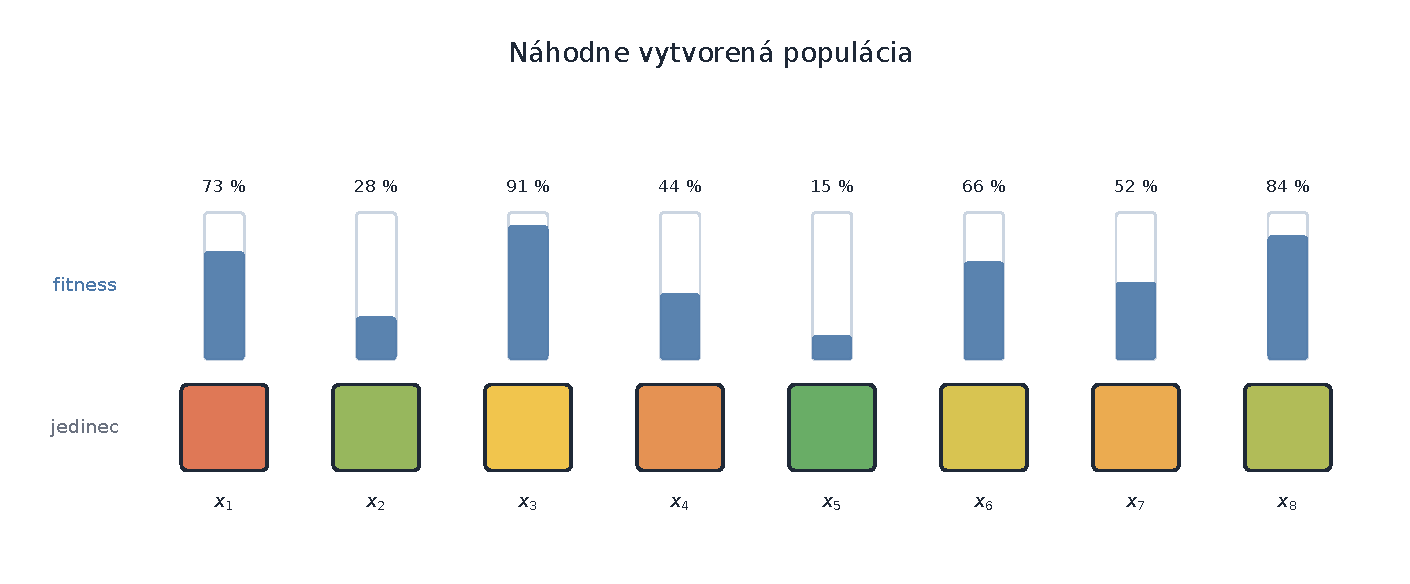
\includegraphics[width=\textwidth]{images/theory/theory_ga_initial_population.pdf}
    \caption[Inicializácia populácie]{Inicializácia populácie genetického algoritmu.}
    \label{fig:ga_initial_population}
\end{figure}

\paragraph{Selekcia rodičov.}
Po vyhodnotení populácie nasleduje výber kandidátov, ktorí budú slúžiť ako rodičia ďalšej generácie. Selekcia môže mať rôzne podoby. Najjednoduchšia predstava je vybrať najlepších kandidátov podľa fitness, ale často sa používa aj pravdepodobnostný výber, aby mali šancu aj slabší jedinci. Takýto prístup môže pomôcť udržať diverzitu populácie a znížiť riziko, že algoritmus príliš skoro uviazne v jednej oblasti priestoru riešení.

Selekcia určuje selekčný tlak. Silný selekčný tlak rýchlo posúva populáciu k aktuálne najlepším riešeniam, ale môže znižovať rozmanitosť. Slabší selekčný tlak ponecháva viac priestoru na prieskum, ale učenie môže byť pomalšie. Tento kompromis bude neskôr dôležitý pri nastavovaní evolučného tréningu.

\begin{figure}[htbp]
    \centering
    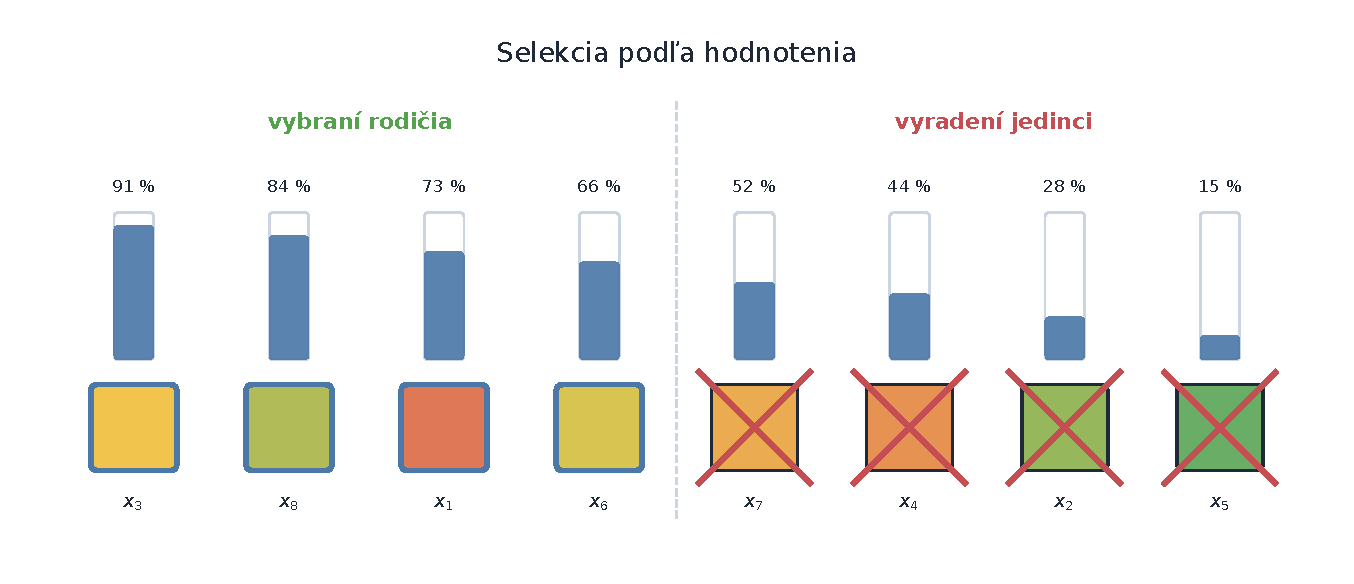
\includegraphics[width=\textwidth]{images/theory/theory_ga_selection.pdf}
    \caption[Selekcia jedincov]{Selekcia jedincov podľa fitness hodnotenia.}
    \label{fig:ga_selection}
\end{figure}

\paragraph{Kríženie.}
Nové riešenia vznikajú z vybraných rodičov pomocou operátorov kríženia a mutácie. Kríženie (angl.~\emph{crossover}) kombinuje časti dvoch alebo viacerých rodičov. Cieľom je vytvoriť potomka, ktorý môže zdediť užitočné vlastnosti z rôznych riešení. V zjednodušenej predstave môžeme rodičov chápať ako už vybrané jedince a výsledkom kríženia je nová generácia potomkov.

\paragraph{Elitizmus.}
Elitizmus znamená, že najlepší kandidáti z aktuálnej generácie sa prenesú do ďalšej generácie priamo alebo s mimoriadnou ochranou. Výhodou je, že algoritmus nestratí už nájdené dobré riešenia náhodnou mutáciou alebo krížením. Nevýhodou môže byť zníženie diverzity, ak elita príliš silno dominuje ďalším generáciám. Elitizmus preto zlepšuje stabilitu hľadania, ale treba ho používať s rozumnou mierou.

Obrázok~\ref{fig:ga_crossover} ukazuje tieto dve myšlienky spolu. Najlepší jedinci môžu prejsť do ďalšej generácie priamo, zatiaľ čo zvyšok novej populácie vzniká krížením vybraných rodičov.

\begin{figure}[htbp]
    \centering
    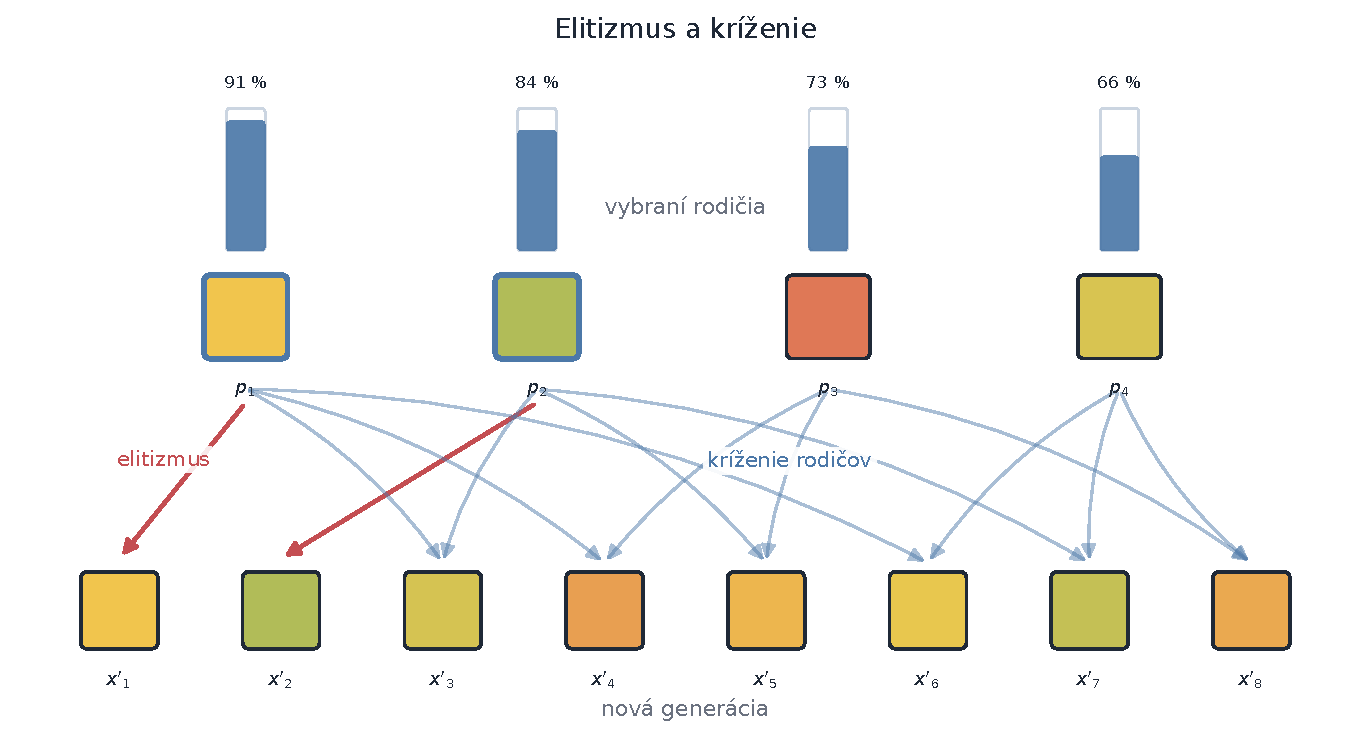
\includegraphics[width=\textwidth]{images/theory/theory_ga_crossover.pdf}
    \caption[Kríženie a elitizmus]{Kríženie rodičov a elitizmus.}
    \label{fig:ga_crossover}
\end{figure}

\paragraph{Mutácia.}
Mutácia zavádza náhodnú zmenu kandidáta. V jednoduchej číselnej reprezentácii ju môžeme zapísať napríklad ako
\[
    x'' = x' + \epsilon,
\]
kde $x'$ je potomok pred mutáciou, $x''$ je potomok po mutácii a $\epsilon$ je náhodná zmena.

Kríženie a mutácia majú rozdielnu úlohu. Kríženie využíva už nájdené čiastkové riešenia, zatiaľ čo mutácia umožňuje objavovať nové oblasti priestoru riešení. Ak je mutácia príliš malá, populácia sa môže prestať výrazne meniť. Ak je príliš veľká, potomkovia môžu strácať dobré vlastnosti rodičov. Aj tu teda vzniká kompromis medzi prieskumom a jemným dolaďovaním.

\begin{figure}[htbp]
    \centering
    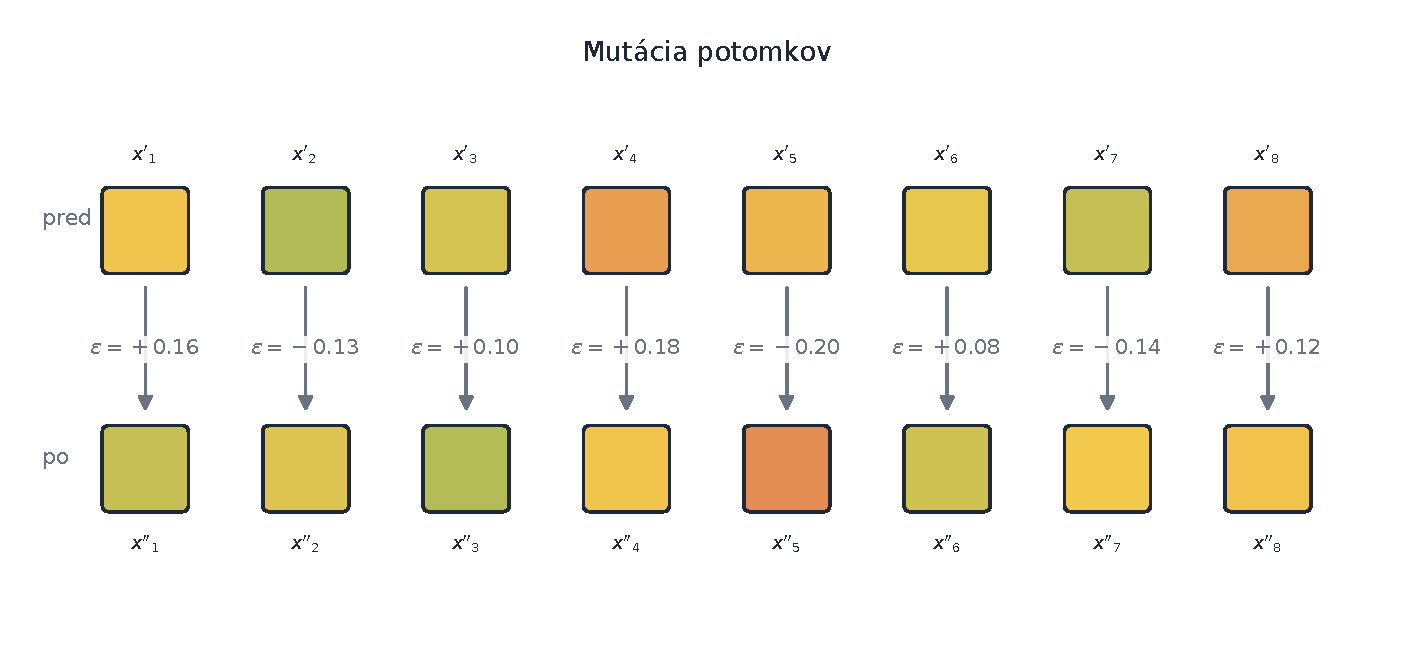
\includegraphics[width=0.9\textwidth]{images/theory/theory_ga_mutation.pdf}
    \caption[Mutácia potomkov]{Mutácia potomkov.}
    \label{fig:ga_mutation}
\end{figure}

\paragraph{Explorácia a dolaďovanie.}
Pri genetických algoritmoch sa často hovorí o explorácii a dolaďovaní. Explorácia znamená hľadanie nových oblastí priestoru riešení. Dolaďovanie znamená menšie úpravy už sľubných riešení. Veľká populácia, vyššia mutácia alebo slabší selekčný tlak môžu podporovať exploráciu. Menšia mutácia a silnejší výber najlepších kandidátov môžu podporovať dolaďovanie.

Tieto pojmy sú dôležité, pretože evolučný algoritmus sa zvyčajne nespráva rovnako počas celého tréningu. Na začiatku môže byť výhodné skúšať veľa odlišných riešení. Neskôr, keď populácia nájde sľubnú oblasť, môže byť výhodnejšie robiť jemnejšie zmeny. V teoretickej rovine ide o rovnaké napätie ako pri prieskume a využívaní znalostí v učení posilňovaním, iba vyjadrené na úrovni populácie kandidátov.

\paragraph{Neuroevolúcia.}
Neuroevolúcia je použitie evolučných algoritmov na neurónové siete. Kandidátom už nie je priamo jedna akcia ani jednoduché pravidlo, ale parametre neurónovej siete. Ak parametre siete označíme ako $\theta$, môžeme kandidáta chápať ako
\[
    x \equiv \theta.
\]
V praxi sú tieto parametre uložené v maticiach váh a vektoroch posunov. Ak ich sploštíme do jedného vektora, dostaneme genóm jedinca, s ktorým môže evolučný algoritmus pracovať podobne ako s iným číselným kandidátom. Túto predstavu znázorňuje obrázok~\ref{fig:neuroevolution_genome}.

\begin{figure}[htbp]
    \centering
    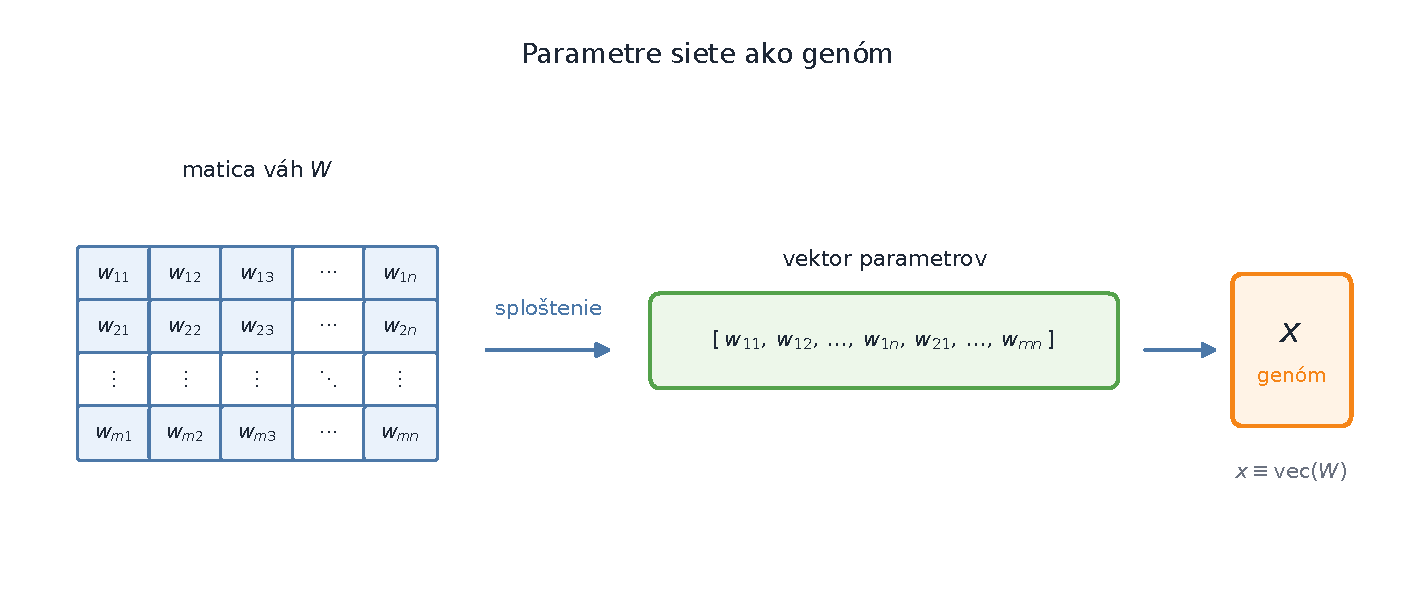
\includegraphics[width=0.92\textwidth]{images/theory/theory_neuroevolution_genome.pdf}
    \caption[Parametre siete ako genóm]{Parametre siete ako genóm pre neuroevolúciu.}
    \label{fig:neuroevolution_genome}
\end{figure}

Vyhodnotenie kandidáta potom znamená spustiť politiku $\pi_\theta$, nechať ju konať v prostredí a ohodnotiť výsledné správanie. Evolučný algoritmus následne vyberá, kombinuje a mutuje celé politiky.

Tento prístup je užitočný najmä vtedy, keď vieme správanie kandidáta vyhodnotiť, ale nechceme alebo nevieme odvodiť gradient cez celé prostredie. Neuroevolúcia sa dá použiť aj na zložitejšie úlohy, kde sa optimalizujú nielen váhy siete, ale aj jej štruktúra. Príkladom je NEAT, ktorý evolučne hľadá váhy aj topológiu neurónovej siete \cite{stanley2002neat}. V tejto práci je dôležitá najmä základná myšlienka: parametre politiky môžu byť priamo kandidátom evolučného hľadania.

\paragraph{Výhody a obmedzenia.}
Výhodou genetických algoritmov je, že nepotrebujú diferencovateľné prostredie ani presný model prechodov. Stačí, aby sme vedeli kandidáta vyhodnotiť. To je praktické pri úlohách, v ktorých je hodnotenie dané celou epizódou alebo obsahuje nespojité udalosti. Genetické algoritmy sú zároveň prirodzene populačné, takže môžu skúmať viacero odlišných riešení naraz.

Obmedzením je počet potrebných vyhodnotení. Ak je jedno vyhodnotenie kandidáta drahé, evolučné hľadanie môže byť časovo náročné. Výsledok je tiež citlivý na reprezentáciu kandidáta, fitness funkciu, veľkosť populácie, mutáciu a selekčný tlak. Genetický algoritmus preto nie je automatická náhrada za návrh problému. Je to nástroj, ktorý môže dobre fungovať vtedy, keď je cieľ rozumne formulovaný a vyhodnotenie kandidátov je uskutočniteľné.

Doteraz sme o fitness hovorili prevažne ako o jednom číselnom hodnotení. V mnohých úlohách však dobré správanie nemožno jednoducho zhrnúť jedným kritériom. Agent môže byť rýchly, ale riskantný. Môže byť bezpečný, ale pomalý. Môže dosiahnuť vysoký krátkodobý progres, ale neskôr zlyhať. Ak má genetický algoritmus vyberať medzi takýmito kandidátmi, musí byť jasné, či ich hodnotíme jednou výslednou hodnotou, pevným poradím priorít alebo množinou samostatných cieľov.

\section{Viackriteriálna optimalizácia}

V predchádzajúcich častiach sme často predpokladali, že kvalitu kandidáta vieme vyjadriť jedným číslom. Takéto hodnotenie je praktické, pretože kandidátov možno jednoducho zoradiť. Pri riadení agenta však často nechceme iba jednu vlastnosť správania. Môže nás zaujímať, či agent dosiahne cieľ, ako rýchlo postupuje, či je jeho správanie stabilné a či sa vyhýba nebezpečným stavom. Tieto ciele nemusia byť vždy v súlade. Viackriteriálna optimalizácia sa zaoberá práve situáciami, v ktorých riešenie posudzujeme podľa viacerých kritérií naraz \cite{coello1999survey}.

\paragraph{Konflikt cieľov.}
Ak máme kandidátne riešenie $x$, jeho kvalitu môžeme opísať vektorom cieľov
\[
    \mathbf{f}(x) = (f_1(x), f_2(x), \ldots, f_k(x)),
\]
kde $f_i$ je $i$-te kritérium a $k$ je počet kritérií. V maximalizačnom zápise chceme, aby boli jednotlivé hodnoty čo najvyššie. V praktických úlohách však zlepšenie jedného kritéria môže zhoršiť iné kritérium. Rýchlejšie správanie môže byť riskantnejšie, bezpečnejšie správanie môže byť pomalšie a riešenie s dobrým krátkodobým výsledkom nemusí byť najlepšie z dlhodobého hľadiska.

Tento konflikt je dôležitý preto, že neexistuje vždy jedno riešenie, ktoré by bolo najlepšie vo všetkých kritériách. Ak také riešenie existuje, výber je jednoduchý. Ak neexistuje, musíme určiť, aký kompromis je pre danú úlohu prijateľný.

\paragraph{Skalárna agregácia.}
Jedna možnosť je previesť viac kritérií na jedno skalárne skóre. Ak jednotlivým kritériám priradíme váhy $w_i$, môžeme písať
\[
    S(x) = \sum_{i=1}^{k} w_i f_i(x),
\]
kde $S(x)$ je výsledné skóre kandidáta. Takýto prístup je jednoduchý a dobre sa používa v optimalizačných algoritmoch, ktoré očakávajú jednu hodnotu. Jeho slabinou je voľba váh. Váhy musia vyjadrovať skutočné priority a zároveň musia rešpektovať rozsahy jednotlivých metrík. Ak sú kritériá v odlišných mierkach, jedno kritérium môže výsledné skóre ovládnuť iba preto, že má väčšie číselné hodnoty.

Skalárna agregácia preto nie je nesprávna, ale musí byť čitateľná a odôvodnená. Ak váhy pôsobia ako ľubovoľné konštanty bez jasnej interpretácie, výsledné správanie môže byť ťažké vysvetliť. Pri agentoch je to obzvlášť citlivé, pretože optimalizačný algoritmus sa bude snažiť využiť presne tú funkciu, ktorú sme mu zadali.

\paragraph{Lexikografické poradie.}
Ďalšou možnosťou je ponechať kritériá oddelené a porovnávať ich podľa pevného poradia priorít. Tento prístup sme už zaviedli pri hodnotení správania agenta ako lexikografické porovnávanie. Vo viackriteriálnej optimalizácii ho môžeme chápať ako špeciálny spôsob rozhodovania: prvé kritérium má najvyššiu prioritu, druhé rozhoduje až pri rovnosti prvého a tak ďalej \cite{ehrgott2005multicriteria}.

Výhodou je, že priority sú jasne vyjadrené poradím kritérií. Nevýhodou je tvrdosť tohto poradia. Ak prvé kritérium rozlišuje kandidátov, nižšie kritériá sa vôbec nedostanú k slovu. Lexikografické poradie je preto vhodné vtedy, keď skutočne vieme povedať, že jeden cieľ má prednosť pred všetkými ostatnými. Ak chceme skúmať širšiu množinu kompromisov, potrebujeme iný pohľad.

\paragraph{Pareto dominancia.}
Pareto dominancia ponúka spôsob, ako porovnávať riešenia bez toho, aby sme museli hneď určiť jednu sadu váh alebo jedno pevné poradie priorít. Pre maximalizačný prípad povieme, že riešenie $x$ dominuje riešenie $y$, ak je aspoň také dobré vo všetkých kritériách a lepšie aspoň v jednom kritériu. Zapíšeme to ako
\[
    x \prec y,
\]
ak platí
\[
    \forall i: f_i(x) \ge f_i(y)
    \quad \text{a zároveň} \quad
    \exists j: f_j(x) > f_j(y).
\]
Prvá podmienka hovorí, že $x$ nie je horšie ako $y$ v žiadnom kritériu. Druhá podmienka hovorí, že v aspoň jednom kritériu je prísne lepšie. Ak ani jedno riešenie nedominuje druhé, znamená to, že každé z nich má inú výhodu a medzi nimi treba urobiť kompromis \cite{coello1999survey}.

\paragraph{Pareto fronta.}
Riešenia, ktoré nie sú dominované žiadnym iným riešením v množine kandidátov, tvoria Pareto frontu. Pareto fronta teda neobsahuje jedno univerzálne najlepšie riešenie, ale množinu kompromisov. Každý bod na fronte je v istom zmysle efektívny: ak chceme zlepšiť jedno kritérium, musíme zhoršiť aspoň jedno iné kritérium.

Pre agenta je tento pohľad prirodzený. Ak hodnotíme napríklad úspešnosť, rýchlosť a bezpečnosť, rôzne politiky môžu predstavovať rôzne štýly správania. Jedna môže byť rýchla a riskantná, druhá pomalšia a stabilnejšia. Pareto fronta umožňuje tieto alternatívy zachytiť bez toho, aby sme ich hneď skryli do jedného čísla.

\paragraph{NSGA-II.}
NSGA-II je známy evolučný algoritmus pre viackriteriálnu optimalizáciu. Používa triedenie podľa nedominovanosti, teda rozdeľuje kandidátov do frontov podľa toho, kto koho dominuje. Okrem toho používa mieru hustoty riešení, často označovanú ako crowding distance, aby v populácii udržiaval diverzitu riešení pozdĺž Pareto fronty \cite{deb2002nsga2}.

V kontexte evolučných algoritmov je to dôležité, pretože nechceme, aby populácia skončila iba pri jednom type kompromisu. Ak optimalizujeme viac cieľov, môže byť užitočné udržať viac odlišných riešení, ktoré reprezentujú rôzne časti fronty. NSGA-II preto nie je iba spôsob výberu najväčšieho čísla. Je to mechanizmus, ktorý sa snaží súčasne zohľadniť kvalitu riešení aj rozmanitosť kompromisov.

\paragraph{Význam pre hodnotenie agenta.}
Viackriteriálna optimalizácia je pre autonómnych agentov dôležitá preto, že dobré správanie má zvyčajne viac rozmerov. Jedno číselné hodnotenie je jednoduché a praktické, ale môže zakryť konflikt medzi cieľmi. Lexikografické poradie dáva jasné priority, ale môže byť príliš tvrdé. Pareto prístup umožňuje skúmať kompromisy, ale konečný výber riešenia stále vyžaduje interpretáciu.

Tým máme opísaný základný optimalizačný rámec správania agenta. Vieme hovoriť o politike, jej parametroch, hodnotení kandidátov aj o situáciách, keď jedno kritérium nestačí. Pri praktickom výskume však tieto pojmy potrebujú aj prostredie, v ktorom možno kandidátne správanie bezpečne a opakovateľne skúšať.

% TODO: doplniť jednoduchý 2D nákres Pareto fronty s dominovanými a nedominovanými riešeniami.

\section{Simulácie a virtuálne prostredia}

Pri učení a vyhodnocovaní agentov nestačí mať iba politiku a hodnotenie. Potrebujeme aj prostredie, v ktorom možno politiku opakovane spustiť, pozorovať dôsledky jej akcií a porovnať ju s inými kandidátmi. Simulácia alebo virtuálne prostredie tu funguje ako kontrolovaný priestor pre experiment: agent dostáva pozorovania, vykonáva akcie a z prostredia vzniká trajektória spolu s metrikami, ktoré vieme zaznamenať.

Takéto prostredia sú dôležité najmä preto, že učenie agenta prirodzene zahŕňa veľa zlých pokusov. V simulácii sú chyby lacné, opakovateľné a dajú sa logovať. Štandardizované prostredia typu OpenAI Gym vznikli práve preto, aby algoritmy učenia posilňovaním dostali spoločné rozhranie a porovnateľné úlohy \cite{brockman2016openai_gym}. V autonómnom riadení podobnú úlohu plnia simulátory, ktoré umožňujú vytvárať kontrolované scenáre pre tréning a vyhodnocovanie jazdných systémov \cite{dosovitskiy2017carla}.

Pre túto prácu sú podstatné najmä dve vlastnosti prostredia: opakovateľnosť a časovanie. Pri opakovateľnosti rozlišujeme najmä \textbf{deterministické} a \textbf{stochastické alebo prakticky variabilné} prostredie. Ak je prostredie deterministické, rovnaký stav a rovnaká akcia vedú k rovnakému ďalšiemu stavu. Takýto prechod môžeme zapísať ako
\[
    s_{t+1} = f_{\text{sim}}(s_t, a_t),
\]
kde $f_{\text{sim}}$ je prechodová funkcia simulácie. Ak je prostredie stochastické alebo prakticky variabilné, výsledok môže závisieť od šumu, počiatočných podmienok, numeriky alebo časovania. Potom prechod opisujeme pravdepodobnostne:
\[
    s_{t+1} \sim P_{\text{sim}}(\cdot \mid s_t, a_t).
\]
Deterministické prostredie je výhodné pri ladení, pretože rovnaký experiment možno presnejšie zopakovať. Variabilné prostredie je náročnejšie na interpretáciu, ale lepšie ukazuje, či je správanie agenta krehké alebo stabilné.

Druhou praktickou otázkou je, či prostredie beží v pevných krokoch alebo v reálnom čase. Z hľadiska časovania teda rozlišujeme \textbf{synchrónne} a \textbf{realtime alebo asynchrónne} prostredie. V synchrónnom prostredí agent vykoná akciu, prostredie spraví jeden krok a až potom vznikne ďalšie pozorovanie. V realtime alebo asynchrónnom prostredí môže medzi dvoma rozhodnutiami uplynúť rôzny čas. Rovnaká akcia preto nemusí mať rovnaký účinok, ak pôsobí dlhšie, kratšie alebo v inom okamihu fyzikálneho výpočtu. Pri riadiacich úlohách je táto vlastnosť dôležitá, lebo politika neovplyvňuje iba smer rozhodnutia, ale aj jeho načasovanie.

\section{Trackmania ako prostredie pre agenta}

Trackmania je cieľové virtuálne prostredie tejto práce. Ide o pretekársku hru, v ktorej je základným cieľom prejsť trať čo najrýchlejšie \cite{ubisoft_trackmania2026}. V režime, ktorý je pre túto prácu dôležitý, nejde o priamy súboj s inými autami na trati. Rozhoduje najmä čas prejazdu a trajektória, ktorou sa hráč alebo agent po trati pohybuje.

Z pohľadu teórie je Trackmania zaujímavá ako úloha sekvenčného rozhodovania v reálnom čase. Auto sa pohybuje priebežne a každá akcia mení stav, z ktorého sa bude rozhodovať v ďalšom okamihu. Rovnaký vstup môže mať iný účinok pri nízkej a vysokej rýchlosti, pred zákrutou a uprostred zákruty alebo pri inom načasovaní. Aj malá odchýlka v brzdení či natočení môže po niekoľkých sekundách znamenať inú stopu na trati.

Trate v Trackmanii majú stavebnicový charakter a môžu obsahovať rôzne tvary, výšky alebo povrchy \cite{trackmania_wiki2026}. V tejto kapitole však tieto prvky stačí chápať iba ako vlastnosti prostredia. Podstatné je, že agent nerieši jednu izolovanú reakciu, ale celú jazdu: musí sa dostať do cieľa, udržať stabilnú trajektóriu a zároveň nestratiť zbytočne veľa času.

Práve tento konflikt robí z pretekárskych hier užitočné prostredie pre skúmanie učiacich sa agentov. Úloha má jasne merateľný cieľ, ale dobré správanie nemožno posúdiť iba z jedného okamihu. Treba hodnotiť celý prejazd, jeho stabilitu, čas a schopnosť neopustiť použiteľnú trajektóriu \cite{offline_mania2024}.

% TODO: doplniť ilustračný náhľad prejazdu trate v Trackmanii: trať, štart, cieľ, trajektória auta a výsledný čas.

\section{Základné pojmy riadenia vozidla a pretekárskej jazdy}

Aj keď ide o hru, slovník jazdy ostáva podobný ako pri všeobecnom riadení vozidla. Pre ďalšie kapitoly nám stačí rozlíšiť pozdĺžne správanie, teda najmä zrýchľovanie a brzdenie, a bočné správanie, teda zatáčanie, stabilitu a pohyb v zákrute. Takéto členenie je bežné aj v literatúre k dynamike vozidiel \cite{rajamani2012vehicle_dynamics}.

Rýchlosť, brzdenie a zatáčanie sú v texte dôležité nie ako samostatné fyzikálne veličiny, ale ako súčasť rozhodovania. Ak agent pridá plyn, brzdí alebo zatočí, účinok tejto akcie závisí od aktuálnej rýchlosti, polohy auta, natočenia a priľnavosti. Rovnaké zatočenie môže byť pri pomalej jazde bezpečné, ale pri vyššej rýchlosti môže viesť k šmyku alebo k nevhodnej polohe pred ďalšou zákrutou.

Rovnako dôležitá je trajektória. Pretekárska stopa nie je iba čiara medzi štartom a cieľom, ale výsledok mnohých nadväzujúcich rozhodnutí. Dobrá stopa môže byť rýchla, ale riskantná; bezpečnejšia stopa môže agentovi nechať viac priestoru na korekciu, ale môže stáť čas. Preto sa kvalita správania pri jazde ukáže až na celom priebehu epizódy, nie na jednej akcii vytrhnutej z kontextu.

\section{Základy počítačovej grafiky pre virtuálne senzory}

Virtuálne prostredie nemusí byť pre agenta reprezentované iba obrazom. Ak máme k dispozícii geometriu sveta, môžeme sa na okolie pýtať priamo: kde je najbližšia plocha, ako ďaleko je prekážka alebo aký tvar má priestor pred agentom. Pre túto prácu je dôležitá práve táto myšlienka. Geometrická reprezentácia umožňuje zložité prostredie zmeniť na menší počet čísel, ktoré opisujú priestorové vzťahy.

\paragraph{Geometria virtuálneho sveta.}
V počítačovej grafike sa objekty často opisujú pomocou bodov, vektorov, transformácií a plôch \cite{dunn2011mathprimer}. Pre agenta nie je dôležité, aby tieto pojmy poznal ako človek. Dôležité je, že program s nimi vie počítať. Ak má objekt vlastný lokálny súradnicový systém, transformácia určuje, kde sa tento objekt nachádza vo svete. V homogénnych súradniciach možno takýto prevod zapísať napríklad ako
\[
    \mathbf{x}_{\text{world}} = T \mathbf{x}_{\text{local}}.
\]
Matica $T$ tu reprezentuje posun, rotáciu alebo mierku objektu. Takýto zápis nie je cieľom sám o sebe; je to spôsob, ako dostať jednotlivé časti sveta do spoločného priestoru, v ktorom sa potom dajú hľadať vzdialenosti a prieniky.

\paragraph{Trojuholníková sieť.}
Povrchy zložitejších objektov sa často reprezentujú ako trojuholníková sieť. Trojuholník je jednoduchá rovinná plocha a väčšie povrchy možno aproximovať skladaním mnohých trojuholníkov \cite{hughes2014computer_graphics}. Takáto sieť môže reprezentovať model objektu, stenu, cestu alebo inú časť virtuálneho prostredia. Čím presnejšie sieť zodpovedá skutočnému tvaru objektu, tým presnejšie možno z nej počítať priestorové vzťahy.

\begin{figure}[htbp]
    \centering
    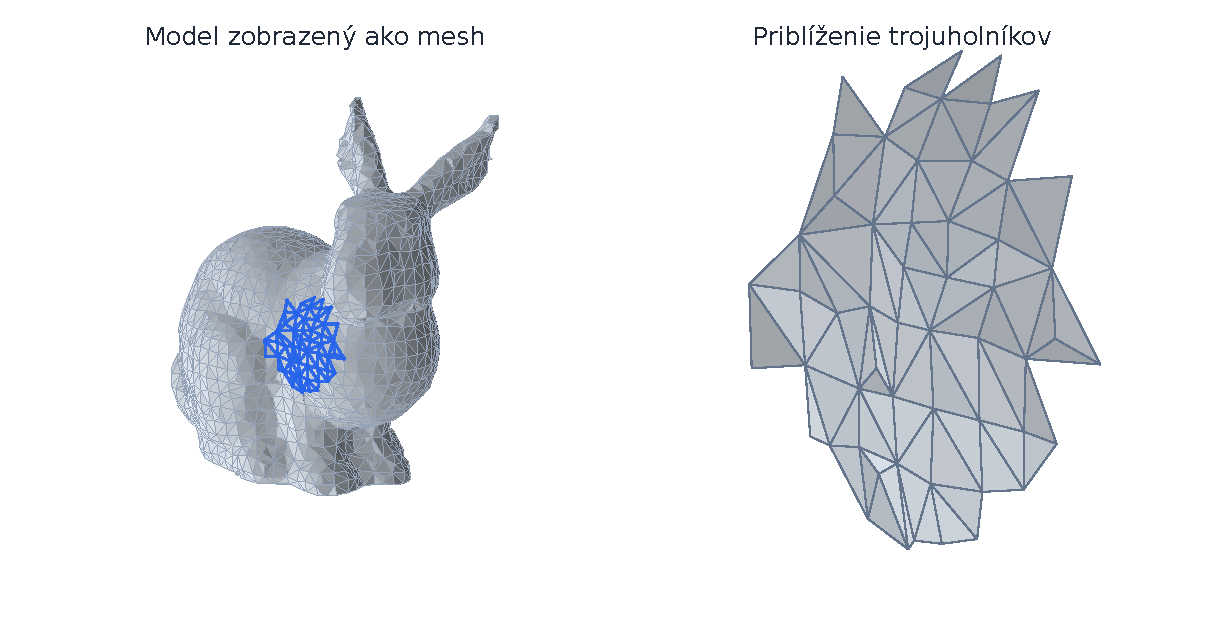
\includegraphics[width=\textwidth]{images/theory/theory_bunny_mesh_overview.pdf}
    \caption[Trojuholníková sieť modelu]{Trojuholníková sieť modelu Stanford Bunny a priblíženie na jej lokálnu štruktúru. Geometria modelu pochádza zo Stanford 3D Scanning Repository, ktorú spravuje Stanford University Computer Graphics Laboratory \cite{stanford3dscanrep2026}.}
    \label{fig:bunny_mesh_overview}
\end{figure}

\paragraph{Raycasting.}
Ak poznáme geometriu sveta, môžeme do nej vyslať lúč a hľadať jeho prvý prienik s povrchom. Lúč je polpriamka so začiatkom v bode $\mathbf{o}$ a smerom $\mathbf{d}$. Zapíšeme ho ako
\[
    \mathbf{r}(t) = \mathbf{o} + t\mathbf{d}, \qquad t \ge 0.
\]
Parameter $t$ určuje vzdialenosť pozdĺž lúča od jeho začiatku. Raycasting potom znamená výpočet, pri ktorom zisťujeme, či lúč pretína geometriu a ktorý prienik je najbližší.

Pri trojuholníkovej sieti je základnou operáciou prienik lúča s jedným trojuholníkom. Algoritmus Möller--Trumbore rieši tento prienik priamo a bez potreby vopred ukladať rovnice rovín jednotlivých trojuholníkov \cite{moller1997raytriangle}. Jeden takýto test je priamy geometrický výpočet. Pri celej sieti však výsledná rýchlosť závisí aj od počtu trojuholníkov a od toho, ako sú dáta v priestore organizované.

\begin{figure}[htbp]
    \centering
    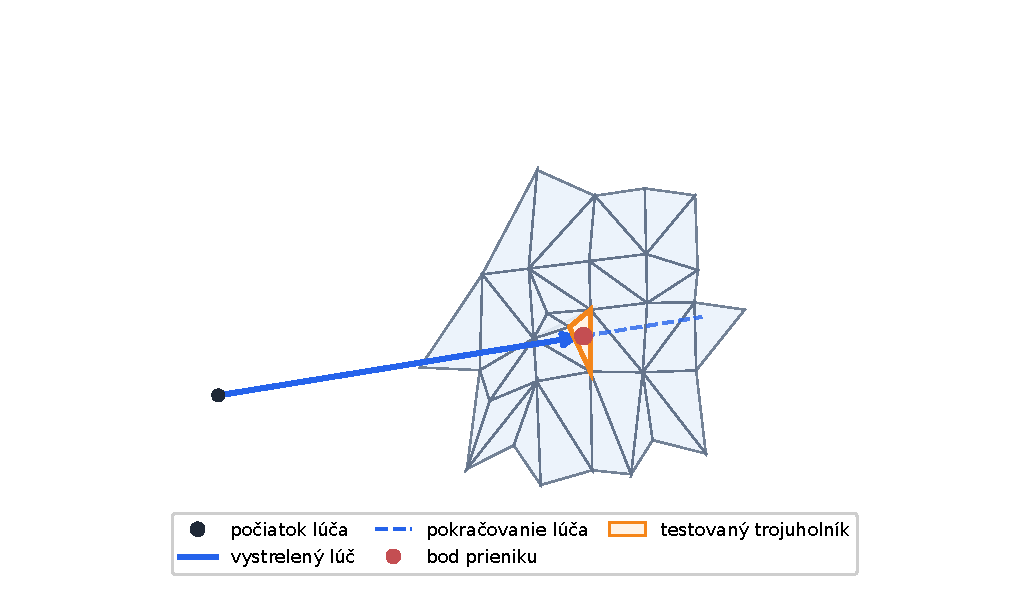
\includegraphics[width=0.82\textwidth]{images/theory/theory_mesh_raycasting_detail.pdf}
    \caption[Raycasting na trojuholníkovej sieti]{Ilustrácia lúča pretínajúceho trojuholníkovú sieť. Zvýraznenie lúča, smeru a prieniku je vytvorené pre túto prácu; použitá geometria modelu Stanford Bunny pochádza zo Stanford 3D Scanning Repository, ktorú spravuje Stanford University Computer Graphics Laboratory \cite{stanford3dscanrep2026}.}
    \label{fig:mesh_raycasting_detail}
\end{figure}

\paragraph{Virtuálne senzory.}
Vo fyzickom svete senzor meria vlastnosť okolia. Vo virtuálnom prostredí môžeme podobný signál vypočítať z geometrie. Ak z jedného bodu alebo z okolia objektu vyšleme viac lúčov rôznymi smermi, vzdialenosti k najbližším prienikom vytvoria kompaktný opis priestoru pred agentom. Výhodou je, že agent nemusí spracúvať celý obraz. Namiesto množstva pixelov dostane menší a ľahšie interpretovateľný vektor čísel.

Tento prístup má aj hranicu. Geometrický senzor vidí iba to, čo je v geometrickom modeli dostupné a dostatočne presné. Nezachytáva všetky vizuálne informácie, ktoré by boli prítomné v obraze, a jeho kvalita závisí od toho, ako dobre je virtuálny svet reprezentovaný. Pre úlohy, kde je dôležitý najmä tvar priestoru, vzdialenosť k prekážkam a poloha voči trati, však môže byť takáto reprezentácia vhodným kompromisom medzi informatívnosťou a jednoduchosťou vstupu.
